% This template has been downloaded from:
% http://www.LaTeXTemplates.com
%
% Original author:
% Frits Wenneker (http://www.howtotex.com)


%----------------------------------------------------------------------------------------
%	PACKAGES AND OTHER DOCUMENT CONFIGURATIONS
%----------------------------------------------------------------------------------------

\documentclass[oneside]{article}
\usepackage{multicol}

\usepackage{lipsum} % Package to generate dummy text throughout this template


\usepackage[T1]{fontenc} % Use 8-bit encoding that has 256 glyphs


\usepackage[hmarginratio=1:1,top=32mm,columnsep=20pt]{geometry} % Document margins
%\usepackage{multicol} % Used for the two-column layout of the document
\usepackage[hang, small,labelfont=bf,up,textfont=it,up]{caption} % Custom captions under/above floats in tables or figures
\usepackage{booktabs} % Horizontal rules in tables
\usepackage{float} % Required for tables and figures in the multi-column environment - they need to be placed in specific locations with the [H] (e.g. \begin{table}[H])
\usepackage{hyperref} % For hyperlinks in the PDF
\usepackage{graphicx}
\usepackage{wrapfig}
%\graphicspath{ {image/} }

\usepackage{lettrine} % The lettrine is the first enlar ed letter at the beginning of the text
\usepackage{paralist} % Used for the compactitem environment which makes bullet points with less space between them

%\usepackage{abstract} % Allows abstract customization
%\renewcommand{\abstractnamefont}{\normalfont\bfseries} % Set the "Abstract" text to bold
%\renewcommand{\abstracttextfont}{\normalfont\small\itshape} % Set the abstract itself to small italic text


\usepackage{titlesec} % Allows customization of titles
\renewcommand\thesection{\arabic{section}} % Arabic numerals for the sections
\renewcommand\thesubsection{\arabic{section}.\arabic{subsection}} % Arabic numerals for subsections
\titleformat{\section}[block]{\large\scshape\centering}{\thesection}{1em}{} % Change the look of the section titles
\titleformat{\subsection}[block]{\large}{\thesubsection}{1em}{} % Change the look of the section titles

\usepackage{fancyhdr} % Headers and footers
\pagestyle{fancy} % All pages have headers and footers
\fancyhead{} % Blank out the default header
\fancyfoot{} % Blank out the default footer
%\fancyhead[C]{Running title $\bullet$ November 2012 $\bullet$ Vol. XXI, No. 1} % Custom header text
\fancyfoot[RO,LE]{\thepage} % Custom footer text

%----------------------------------------------------------------------------------------
%	TITLE SECTION
%----------------------------------------------------------------------------------------

\title{\vspace{-20mm}\fontsize{20pt}{10pt}\selectfont\textbf{Stuck in Traffic \\Intermediate Report}}
\author{
\large
{Antria Dimitriou, Filippo Mariani, Maximilian Nikolaidis, Filippos Raditsas, Maxim Vasilishin}\\[10mm] % Your name
%\normalsize King's College London \\ [10mm] % Your institution
%\normalsize \href{mailto:filippo.mariani@kcl.ac.uk}{filippo.mariani@kcl.ac.uk} % Your email address
\vspace{-85mm}
}
\date{}

%----------------------------------------------------------------------------------------

\begin{document}

\maketitle %add title

%\thispagestyle{fancy} % All pages have headers and footers

%----------------------------------------------------------------------------------------
%	ABSTRACT
%----------------------------------------------------------------------------------------

%\begin{abstract}

%\noindent \lipsum[0]  % Dummy abstract text

%\end{abstract}

%\clearpage 
%----------------------------------------------------------------------------------------
%	ARTICLE CONTENTS
%----------------------------------------------------------------------------------------

%\begin{multicols}{2} % Two-column layout throughout the main article text

\section{Introduction}

In this intermediate report we will present our initial idea about the traffic management simulation software we will design and build. Road traffic management is a well known problem in such big city like London. In the last few years a lot of research has been driven by the importance of improving traffic management in the best way possible. Our idea is to ultimately create a simulation platform that will be fully customizable by the users and will allow them to simulate the scenarios of their preference. We will be using Java in Eclipse IDE as our main programming language and Photoshop for the creation of the graphics.

\section{Project Description}

The aim of this project is to develop a simulation engine, which could be utilized for testing scenarios and potentially improve the well known issue of traffic management and optimization. Our goal is to have abstract concepts that will allow us to simulate certain scenarios but also become an easy adaptive platform to build on top for future ideas. Our first level aim is to develop a platform which loads a map, identifies possible paths for the cars, supports two way vertical and horizontal roads, as well as intersections. The map has entry points and exit points; upon arrival to an exit point the car object will be deleted. Our initial model will have a car, which is going to follow all the possible paths of our sample map. The next step will be to add more cars onto the map, as well as traffic lights to control the traffic. If time allows it, we are planning to have multi-lane roads and support scenarios of different driving behaviors such as reckless driving, too slow driving and cases of "polite" drivers that give way to other cars in order to help the road's decongestion. Furthermore ideas for future implementation also include parking spots, emergency lanes and vehicles, as well as pedestrians crossing the road. 
%For this group project we will implement and simulate some of the most common scenarios that can be experienced during a normal day. The simulation will present a scenario where two or more vehicles meet at an intersection and we will simulate how the traffic lights handle such scenarios to control traffic. The aim of the project is to have a first understanding of the problem faced by road traffic enforcement. The simulation will try to provide a solid starting block to further simulations and observations. For this reason users will be allowed to create their own maps. Upon initialization of our simulator and the choice of a map all possible paths are going to be calculated and all the cars entering the grid will have predefined randomly chosen starting and ending point as well as a path that they will follow. 

%\subsection{Description of Simulation Platform}
%In its final version, our platform will generate a grid in which users can enter roadblocks in order to create their maps. After each roadblock is placed in the grid, every possible next step is defined automatically. For example, if a user places a horizontal roadblock, the next possible roadblock cannot be a vertical, but another horizontal or an intersection roadblock. That way we implement rules for the map creation and make the process user friendly. Upon placement of all the roadblocks, the map can be saved and reused at a later time. For a complete map that is selected the grid is analyzed automatically and all the possible paths the cars could follow are determined; the user can also decide on the number of cars that enter the map per certain number of ticks, as well as the utilization of a specific path in order to simulate certain traffic scenarios. So this way the user has created his map and defined the simulation scenario he wishes to execute. 

\subsection{Technical Challenges}
Since we decided to use Java, we also had to think about the animation which requires repaint of the graphics so that the movement of the cars is smooth. To avoid performance issues and large memory consumption we will have to write a function which takes as a parameter the size and number contents of the grid and decides what's the optimal repaint time threshold. Additionally, in order to avoid implementing car to car communication algorithms and A.I, we decided to follow a predefined-path approach for the cars in the simulation. That way we allow the users to customize the simulation according to their needs instead of simulating a specific pseudorandom scenario that would be limited by the efficiency of our algorithms. Apart from that, we considered implementing more sophisticated methods infeasible for the timeframe given for this project.

%\lettrine[nindent=0em,lines=3]{L} orem ipsum dolor sit amet, consectetur adipiscing elit.
%\lipsum[0] % Dummy text

 %\subsection{Ideas and Future Work}
%If the intended tasks have been completed , add-on components will be :

\section{Strategy, Timetable, and Progress}

\noindent Stuck in traffic will use the expertise of each member in each phase of the project in order to complete all required tasks. Our goal is to exchange knowledge and build not only a great traffic simulator but also develop teamwork skills. %Our solution will provide users with a list of maps from which they can choose one to perform their simulation, as well as customize the number of cars and other parameters. In order to deliver this task we aim to provide users with good quality User Experience Design (UEX).

\subsection{Team Member Roles}

\noindent The lead of each phase is listed below, although all members will collaborate during all phase of this project.  

\begin{itemize}
\setlength\itemsep{-0.5em}
\item Project coordinator: Filippos Raditsas
\item Analysis: Filippo Mariani
\item Software Architecture Design/Development: Maxim Vasilishin
\item Graphics and GUI Design \& Development: Maximimilian Nicolaidis, Antria Dimitriou
\item QA: Antria Dimitriou
\end{itemize}

\noindent \textbf{Analysis:} The analysis phase included a feasibility assessment in which possible technologies, programming languages and solution approaches were evaluated. During this process all members collaborated and brought their thoughts and opinions to the table in order to finalize our idea and further proceed with the project.\\
\newline
\noindent \textbf{Software Architecture Design/Development:} This team is responsible for the high level design of the project, assisting in the transition from requirements to technical specifications leading to the development. They will take up tasks broken down by the lead developer. During the initial stage of our project our lead developer has managed to build an initial version of our simulation platform upon which we'll build the rest of the functionality.\\
\newline
\noindent \textbf{Graphics and GUI Design:} This team will work on the GUI that we will integrate to our platform in order to make it interactive. The design team also provided the graphics that are used in our simulator including but not limited to roads, cars and traffic lights.\\ 
\newline
\noindent \textbf{QA Testing:} The responsibilities of the Quality Assurance team will be testing the simulator to ensure all components work smoothly are and consistent with the specifications and requirements. All the bugs found will be reported to the development team and if changes are necessary they will be handed over to the analysis team to perform a requirements analysis.

%\noindent In order to maintain a proper time management we have created a gantt chart. The chart will be used in order to set internal deadlines and to have a more accurate and fair workflow distribution among our group during the project time. 
\begin{figure}[h]
\centering
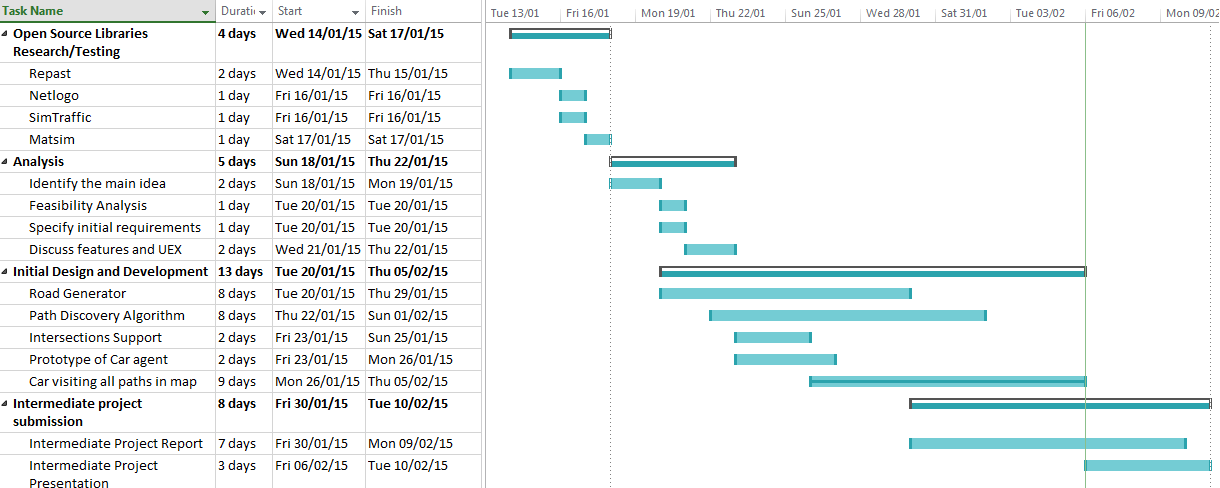
\includegraphics[width=6in]{ganttchart}
\caption{Gantt Chart depicting main tasks and rough timetable for intermediate report}
\end{figure}

\subsection{Methodology}
 
Our team follows the Spiral model which is a risk driven process. We believe that the spiral model is more appropriate for this kind of project, as it will help us mitigate risks such as steep learning curve during the development phase, limited time, individual member's unforeseen circumstances and enable us to add features and ideas to the project. We have divided the spiral model in 4 main phases: 

 \begin{itemize}
 \setlength\itemsep{-0.5em}
  \item Requirements Analysis: We investigated available open source libraries and formed our idea. 
  \item Risk Analysis: We will constantly evaluate the risk during the different phases of the project. 
  \item  Development: After the initial risk analysis we start developing our project divided in tasks.
  \item  Evaluation: We will maintain proper documentation and implementation requirements of each task. 	  	  
 \end{itemize}
 
\begin{figure}[h]
\centering
\includegraphics[width=4.5in]{spiralFINALv2}
\caption{Spiral Model}
\end{figure}

\section{Conflict resolution procedure}

\noindent The resolution will contain three phases which will be executed linearly.

\noindent \textbf{Phase 1:} Group members will make every effort to resort minor disputes in a civilized manner, discussing their issue with the team, individual. Team members do have other responsibilities, schedules outside of this project and members need to take that into consideration and respect each other. However if the issue is not resolved then the issue will be escalated to phase 2.\\
\newline
\noindent \textbf{Phase 2:} The group member with the issue will at this point fill out a conflict resolution form, which will be provided by the team with the intent of helping resolve any issue. The form includes the members name, issue with certain member or aspect of the group, and how this issue will be resolved. The member will then email the form to all other members of the group to arrange a meeting discussing the issue. Meeting minutes are going to be kept for further proof, at this point if the issue is not then resolved the member can further escalate it to phase 3.\\
\newline
\noindent \textbf{Phase 3:} In Extreme cases of fraud or ill reference allegation towards any group member, the member has the right to be in correspondence with the professor on behalf the individual. The member with the issue \textbf{must} contact the professor via email and cc every group member in the email. Depending on the response of the professor the team will then once again meet with the member to resolve the issue as quickly as possible. This process will be recorded on a conflicted resolution form, a copy will be sent to all individuals in the team.

\begin{figure}[h]
\centering
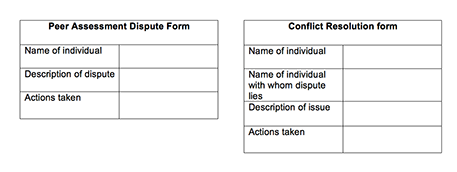
\includegraphics[width=4in]{both}
\caption{Conflict Resolution and Peer Assessment}
\end{figure}

\section{Peer assessment}
\noindent The peer assessment takes place to ensure a fair distribution of points for each member upon completion of the project. The amount of points awarded to a particular member may alter based on their contribution to the project and amount of work they put towards helping other members. Since there are five members in the team and there are 100 points to give accordingly the ultimate goal of our team is to evenly distribute the points assuming that we will all contribute the same amount of work and will collaborate smoothly and efficiently.
\newline

\noindent In the event that a team member wishes to dispute their given peer assessment, they would need to raise the issue with the whole team. The individual would fill out a Peer Assessment Dispute Form, which includes the individuals name, brief description of dispute and the actions taken. After the team has decided the outcome of the individual, the new assessment for that individual will be regarded as final, no further disputes can be made. 

\subsubsection{Team file management}
We are required to work as team for the whole time of the project. For code sharing we have a Github repository.
For our internal communication purposes: 
 \begin{itemize}
  \item Slack Framework: https://slack.com/ We have created a group account to communicate and exchange files. 
  \item Skype Conference: http://www.skype.com/en/ We have created an internal schedule for online meetings. 
  \item Physical Meetings:We also all meet once a week to discuss any issues.  
 \end{itemize}


%\Copyright \copyright\; 2013 my name\\

%\caption[GantChart]{Gant Chart}


%\section{Our Idea: } %Intelligent traffic with proactive communications



%----------------------------------------------------------------------------------------
%	REFERENCE LIST
%----------------------------------------------------------------------------------------

%\begin{thebibliography}{99} % Bibliography - this is intentionally simple in this template

%\bibitem[Figueredo and Wolf, 2009]{Figueredo:2009dg}
%Figueredo, A.~J. and Wolf, P. S.~A. (2009).
%\newblock Assortative pairing and life history strategy - a cross-cultural
%  study.
%\newblock {\em Human Nature}, 20:317--330.
 
%\end{thebibliography}

%----------------------------------------------------------------------------------------

%\end{multicols}

\end{document}
